\documentclass[serif,mathserif]{beamer}
\usepackage{amsmath, amsfonts, epsfig, xspace}
\usepackage{algorithm,algorithmic}
\usepackage{pstricks,pst-node}
\usepackage{multimedia}
\usepackage[normal,tight,center]{subfigure}
\setlength{\subfigcapskip}{-.5em}
\usepackage{beamerthemesplit}
\usetheme{lankton-keynote}

\author[Payload mask]{ Tool designed for bypass waf \quad 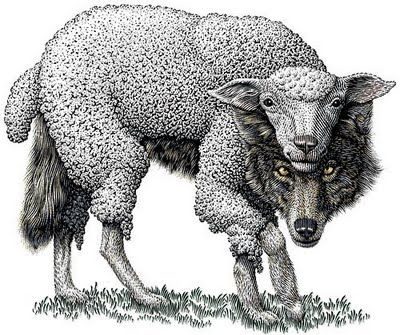
\includegraphics[width=3cm]{images/loboovelha.jpg} }

\title[ Page \hspace{2em}\insertframenumber/\inserttotalframenumber]{Payload mask}

\date{February 8, 2015} 

\institute{Antonio Costa - CoolerVoid - coolerlair[aT]gmail[DOt]com}

\begin{document}

\maketitle

% \section{Introduction}  % add these to see outline in slides



\begin{frame}
  \frametitle{Whoami}
  Author:
  \begin{itemize}  \item  Antonio Costa "CoolerVoid" is a Computer Programmer who loves the Hacker culture, he work as system analyst at CONVISO for three years. Nowadays, Antonio working with code review, pentest and security research with focus on Secure Web Applications and Reverse Engineering and he has speaking in some Brazilian Security Conferences such as YSTS, OWASP Florianopolis and Bsides Sao Paulo.
  \end{itemize}
  \begin{figure}[t]
    \centering
    \subfigure[]{
%    \includegraphics[width=3cm]{figures/naked_leaves/00000240}}
    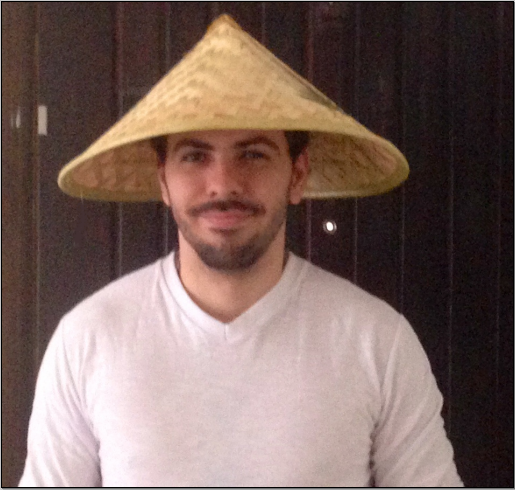
\includegraphics[width=4cm]{images/tony.png}}
  \end{figure}
\end{frame}


\begin{frame}
  \frametitle{Introduction}
  Software Information:
  \begin{itemize}
  \item  Payload mask is a Open Source Tool to generate payload list to try bypass Web Application Firewall, you can use a lot list of encodes and techniques to convert your payload list. 
  \item  Payload mask held by GPL v3 license: https://github.com/CoolerVoid/payloadmask/blob/master/LICENSE.txt
  \end{itemize}
\end{frame}



\begin{frame}
  \frametitle{Introduction}
  Why this tool is made in C language ?
  \begin{itemize}
  \item  C have a high delay time for writing and debugging, but no pain no gain, have a fast performance, addition of this point, the C language is run at any architecture like Mips,ARM and others... at the future can follow mobile implementations. other benefits of C,  have good and high profile to write optimizations, if you think write some lines in ASSEMBLY code with AES-NI or SiMD instructions, i think is good choice. 
  \item  Why you not use POO ? in this project i follow "KISS" principe: http://pt.wikipedia.org/wiki/Keep\_It\_Simple
  \item  C language have a lot old school dudes like a kernel hackers... 
  \end{itemize}
\end{frame}



\begin{frame}
  \frametitle{Introduction}
  Requirements:
  \begin{itemize}
  \item  Need "GCC" and "make" 
  \item  Current version tested only Unix Like systems(Linux, MacOS and *BSD).
  \item  Current version run well, but is a BeTa version, you can report bug here: https://github.com/CoolerVoid/payloadmask/issues
  \end{itemize}
\end{frame}

% \section{Main Body} % add these to see outline in slides

\begin{frame}
  \frametitle{How you can use it}
  Following this to get, decompress, compile and execute:
  \begin{itemize}
  \item wget https://github.com/CoolerVoid/payloadmask/archive/master.zip; 
  \item unzip master.zip; cd payloadmask-master; make; ./payloadmask
  \end{itemize}
\end{frame}



\begin{frame}
  \frametitle{The Overview}
  \begin{figure}[]    
    \centering
    \includegraphics[width=14cm]{images/codeview.png} 
  \end{figure}
\end{frame}


\begin{frame}
  \frametitle{Explain}
  WAF stands for Web Application Firewall. It is widely used nowadays to detect and defend SQL Injections and XSS...
  \begin{itemize}
  \item You can use comments to bypass WAF: http://www.site.com/index.php?page\_id=-15 /*!UNION*/ /*!SELECT*/ 0,1,2,3... 
  \item You can also change the Case of the Command: http://www.site.com/index.php?page\_id=-15 UnIoN sELecT 0,1,2,3...
  \item You can combine methods: http://www.site.com/index.php?page\_id=-15 /*!uNIOn*/ /*!sElECt*/ 0,1,2,3….
  \end{itemize}
\end{frame}


\begin{frame}
  \frametitle{The End}
  \begin{figure}[]    
    \centering
    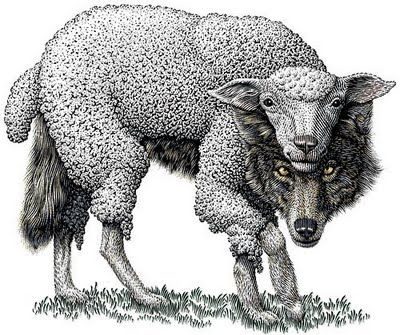
\includegraphics[width=6cm]{images/loboovelha.jpg} 
  \end{figure}
\end{frame}



% \section{Conclusion} % add these to see outline in slides

\begin{frame}
  \frametitle{Greets}
  \begin{itemize}
  \item IAK, Sigsegv, M0nad, Slyfunky , RaphaelSC, pl4nkton, gustavoRobertux, Muzgo, Mente binaria, Otacon...
  \item HB, F-117, Eremita, Clandestine, Loganbr, Geyslan, Clodonil Trigo...
  \item my parents and friends...
  \item https://conviso.com.br/index.php/EN
  \end{itemize}
\end{frame}

\begin{frame}
  \frametitle{at construction...}
\end{frame}

\end{document}
